\section*{Cíle laboratorního cvičení}
\begin{itemize}
  \item Seznámení se se signalizačním protokolem SIP.
  \item Peer-to-peer VoIP pomocí signalizace SIP.
  \item Komunikace VoIP pomocí signalizace SIP přes ústřednu.
\end{itemize}

\section*{Základní instrukce}
\begin{itemize}
  \item Pro práci ve cvičení budete používat následující virtuální stroje v~programu VirtualBox:
  \begin{itemize}
	\item \textbf{PC-A}: První klient (Jitsi).\\
	Virtuální stroj: \url{https://nes.fit.vutbr.cz/isa/ISA2020.ova}
	\begin{table}[H]
		\centering
		\begin{tabular}{|c|c|}
		\hline
		\textbf{Uživatelské jméno} & \textbf{Heslo} \\ \hline
		root                       & root4lab       \\ \hline
		user                       & user4lab       \\ \hline
		\end{tabular}
	\end{table}

	\item \textbf{PC-B}: Druhý klient (Jitsi).\\
	Virtuální stroj: PC-B vytvoříte v~průběhu laboratoře klonováním PC-A dle návodu níže.
	\begin{table}[H]
		\centering
		\begin{tabular}{|c|c|}
		\hline
		\textbf{Uživatelské jméno} & \textbf{Heslo} \\ \hline
		root                       & root4lab       \\ \hline
		user                       & user4lab       \\ \hline
		\end{tabular}
	\end{table}
	\item \textbf{PC-U}: Ústředna (Asterisk).\\
	Virtuální stroj: \url{http://nes.fit.vutbr.cz/isa/isa-asterisk.ova}
	\begin{table}[H]
		\centering
		\begin{tabular}{|c|c|}
		\hline
		\textbf{Uživatelské jméno} & \textbf{Heslo} \\ \hline
		root                       & root       \\ \hline
		isa                       & isa       \\ \hline
		\end{tabular}
	\end{table}
  \end{itemize}
  \item Pokud z~předchozích cvičení máte provedeny nějaké změny ve virtuálních strojích, obnovte je do výchozího stavu.
  \item Před zahájením cvičení si vytvořte snapshoty virtuálních strojů za pomoci
  menu \textit{Machine $\rightarrow$ Take snapshot} pro snadný návrat k~výchozímu stavu.
  \item Odpovědi pište do odpovědního archu \texttt{protokol4.docx}, který odevzdáte do WIS-u ve formátu \texttt{pdf}.
  Dostupný je na adrese\\
  \url{https://github.com/nesfit/ISA/blob/master/voip/protokol/protokol4.docx}.\\
  Pokud nemáte nainstalovaný program Microsoft Word, je možné ze skladu dokumentů ke kurzu ISA stáhnout \texttt{protokol4} i ve formátu \texttt{pdf}.
  \item Do WIS-u budete také odevzdávat všechny zachycené \texttt{pcap} soubory.
\end{itemize}


\section{Příprava prostředí pro VoIP}

\subsection{Instalace Jitsi SoftPhone na PC-A}
\begin{enumerate}
  \item Jitsi SoftPhone je aplikace, která simuluje chování fyzického IP telefonu.
  
  \item Pro instalaci Jitsi SoftPhone na CentOS 7 je nejdříve potřeba vyřešit problém se závislostmi na požadované RPM balíčky.
  Na PC-A zadejte postupně následující příkazy (nekopírujte konce řádků v dlouhých odkazech ze zadání -- odkazy zadávejte do terminálu souvisle bez konce řádku):\footnote{Zdroj: \url{https://github.com/jitsi/jitsi/issues/425#issuecomment-345938823}}
      
	\begin{verbatim}
	rpm -e --nodeps speex
	
	wget https://copr-be.cloud.fedoraproject.org/results/fedpop/speex/
	epel-7-x86_64/00146973-speex/speex-1.2-0.23.rc2.el7.centos.x86_64.rpm
	
	rpm -i speex-1.2-0.23.rc2.el7.centos.x86_64.rpm
	
	wget https://copr-be.cloud.fedoraproject.org/results/fedpop/speexdsp/
	epel-7-x86_64/00146970-speexdsp/speexdsp-1.2-0.7.rc3.el7.centos.x86_64.rpm
	
	rpm -i speexdsp-1.2-0.7.rc3.el7.centos.x86_64.rpm
	\end{verbatim}
	
  \item Následně spusťte lokální instalaci Jitsi SoftPhone na PC-A příkazem:
  
  \verb{yum localinstall https://github.com/jitsi/jitsi/releases/download/Jitsi-2.10/{\\
  \verb{jitsi-2.10-5550.x86_64.rpm{
  
  \item V~případě problémů se stažením RPM balíčku z~oficiálního zdroje, můžete zkusit instalaci z~alternativního zdroje příkazem:\\
  \verb{yum localinstall http://rover.borec.cz/jitsi-2.10-5550.x86_64.rpm{
  
  \item Pokud instalace selže (např. chyba související s~Python), obnovte virtuální stroj do výchozího stavu (ze snímku vytvořeného před začátkem laboratoře) a pokuste se o~instalaci Jitsi ještě jednou.
  
  \item Úspěch instalace ověřte spuštěním aplikace Jitsi příkazem \texttt{jitsi \&}.
  
  \item Vypněte virtuální počítač PC-A.
  
  \item V~programu VirtualBox klikněte pravým tlačítkem na PC-A a zvolte \textbf{Settings $\rightarrow$ Audio} a pokud ještě nejsou, zaškrtněte oba checkboxy (\textbf{Enable Audio Output, Enable Audio Input}) a potvrďte kliknutím na \textbf{OK}. Tento krok je nutný, i když nebudete fyzické audio zařízení používat. Pokud Jitsi nebude mít přístup k~audio zařízení, nenaváže hovor.
\end{enumerate}
  

\subsection{Vytvoření virtuální LAN a připojení PC-A a PC-U do ní}
\begin{enumerate}
  \item Ujistěte se, že PC-A i PC-U jsou vypnutá.
  \item V~programu Virtual Box klikněte na \textbf{Tools $\rightarrow$ Preferences $\rightarrow$ Network $\rightarrow$ Zelené plus (Adds new NAT network)}. Tím vznikne nová virtuální LAN s~názvem \emph{NatNetwork}. Potvrďte kliknutím na tlačítko \textbf{OK}.
  \item Do nově vzniklé virtuální LAN připojte PC-A tak, že kliknete pravým tlačítkem na PC-A a zvolte \textbf{Settings $\rightarrow$ Network}. Zde se ujistěte, že je povolený síťový adaptér a z~rozbalovacího menu \textbf{Attached to:} vyberte \texttt{NAT Network}. A~z~rozbalovacího menu \textbf{Name} vyberte \texttt{NatNetwork}, což je vaše virtuální LAN vytvořená v~předchozím kroku.
  \item Stejným postupem připojte do stejné virtuální LAN také PC-U.
\end{enumerate}


\subsection{Klonování PC-A a vytvoření jeho klonu PC-B}
\begin{enumerate}
	\item Před klonování PC-A se ujistěte, že je PC-A vypnutý.
	\item V~programu VirtualBox klikněte pravým tlačítkem myši na váš virtuální počítač PC-A a vyberte \textbf{Clone...}.
	\item Z~rozbalovacího menu \textbf{MAC Address Policy:} vyberte \texttt{Generate new MAC addresses for all network adapters}. Klikněte na tlačítko \textbf{Další}, změňte \textbf{Full clone} na \textbf{Linked clone} a potvrďte kliknutím na tlačítko \textbf{Clone}.
	\item Nově vzniklý klon je váš PC-B.
	\item Ověřte, že i PC-B má v~programu Virtual Box povolený audio vstup a výstup a že je připojený do virtuální LAN.
\end{enumerate}


\subsection{Ověření konektivity mezi vertuálními počítači}
\begin{enumerate}
	\item Spusťte všechny 3 virtuální počítače (PC-A, PC-B, PC-U). Do počítačů PC-A a PC-B se přihlašte jako uživatel \texttt{user} a do počítače PC-U se přihlašte jako uživatel \texttt{isa}.
	\item Na všech třech počítačích spusťte terminál (na PC-U nastartuje terminál automaticky jako hlavní uživatelské rozhraní) a pomocí příkazu \verb{ip address{ (respektive \verb{ifconfig{ na PC-U) zjistěte IPv4 adresu na rozhraní \emph{enp0s3} (respektive \emph{em0} na PC-U). IPv4 adresy včetně masky sítě v~notaci CIDR (tj. číslo za lomítkem) jednotlivých strojů zapište do protokolu.
	\item Otestujte konektivitu mezi všemi virtuálními počítači pomocí příkazu \verb{ping{. Výsledky zapište opět do protokolu do předpřipravené tabulky.
\end{enumerate}


\section{Peer-to-peer VoIP pomocí signalizace SIP}
Nastavte komunikaci VoIP mezi virtuálními stroji PC-A a PC-B bez použití ústředny (spojení peer-to-peer).

\begin{enumerate}
    \item Na PC-A spusťte program Jitsi příkazem \texttt{jitsi \&} a vyčkejte, až se spustí okno programu.
	V~menu {\bf Tools} $\rightarrow$ {\bf Options} $\rightarrow$ {\bf Accounts} přidejte nový účet. Pro ten nastavte pole {\bf Network} na hodnotu {\tt SIP} a následně {\bf SIP id} na hodnotu {\tt PC-A}, potvrďte tlačítkem \textbf{Add} a zkontrolujte, že se vytvořil \emph{RegistrarLess SIP} účet.
    \item Stejný postup jako v~předchozím bodě zopakujte pro PC-B, kde ale nastavte {\bf SIP id} na hodnotu {\tt PC-B}.
	\item Na PC-B v hlavním okně programu Jitsi zadejte do pole {\bf Enter name or number} IPv4 adresu virtuálního stroje PC-A.
	Z~PC-B zavolejte na PC-A stisknutím tlačítka zeleného telefonu. Napoprvé se pravděpodobně nepodaří hovor navázat, další pokus v~obráceném směru volání by však již měl být úspěšný.
	Hovor ukončete.
	\item Na PC-A i PC-B spusťte síťový analyzátor Wireshark jako uživatel \texttt{root} a začněte zachytávat pakety na rozhraní \emph{enp0s3}.
    \item Po spuštění nastavte display filtr tak, aby zobrazoval pouze protokol SIP (\textbf{Display filter:} \texttt{sip}).
    \item Na PC-A v hlavním okně programu Jitsi zadejte do pole {\bf Enter name or number} IPv4 adresu virtuálního stroje PC-B.
    \item Z~PC-A zavolejte na PC-B stisknutím tlačítka zeleného telefonu. Na počítači PC-B přijměte hovor.
	\item Pokud v~průběhu hovoru kliknete na tlačítka \textbf{Confirm} pro potvrzení bezpečnostního kódu, dojde k~zabezpečení komunikace a změny z~protokolu \texttt{RTP} na protokol \texttt{SRTP} (Secure Real-time Transport).
	\item Po chvíli hovor ukončete.
	\item Po ukončení hovoru zastavte zachytávání provozu v~programu Wireshark na obou počítačích.
	\item Zachycenou komunikaci uložte do souborů \texttt{cv4-p2p-pcA.pcap} a \texttt{cv4-p2p-pcB.pcap}. Tyto soubory budete odevzdávat.
    \item Buď na PC-A nebo na PC-B proveďte analýzu spojení ve Wiresharku. Využijte podpory v~menu {\bf Telephony $\rightarrow$ VoIP Calls}, kde uvidíte jednotlivé zaznamenané hovory (měli byste vidět pouze jediný hovor). Vyberte příslušný hovor a pro zobrazení průběhu klikněte na tlačítko {\bf Flow Sequence}.
    \item Zakreslete spojení do grafu v~protokolu. Uveďte, pomocí kterých protokolů a mezi jakými IP adresami a porty probíhá signalizace a přenos dat. Zjistěte použitý kodek pro přenos hlasu.\\

Názvy a čísla podporovaných kodeků lze zobrazit v SIP/SDP zprávě v sekci {\bf Session Initiation Protocol} $\rightarrow$ {\bf Message body} $\rightarrow$ {\bf Session description protocol}:
\begin{figure}[H]
  \centering
  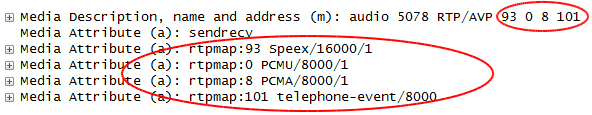
\includegraphics[width=145mm]{img/3a.png}
\end{figure}

\noindent Informace o~tom, který z podporovaných kodeků byl skutečně použit, získáte z RTP paketů (\textbf{Display filter:} \texttt{rtp}) podle čísla v poli {\bf Payload type}.
\begin{figure}[H]
  \centering
  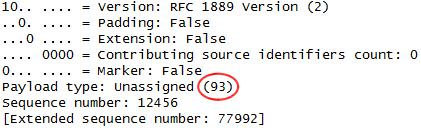
\includegraphics[width=105mm]{img/3b.png}
\end{figure}


    \item Na PC-A i PC-B odstraňte vytvořený \emph{RegistrarLess SIP} účet v~menu {\bf Tools} $\rightarrow$ {\bf Options} $\rightarrow$ {\bf Accounts}.
    \item Na PC-A i PC-B ukončete a znovu spusťte program Jitsi.
\end{enumerate}

\section{Komunikace VoIP pomocí signalizace SIP přes ústřednu}
Nastavte komunikaci VoIP mezi virtuálními stroji PC-A a PC-B pomocí SIP ústředny na virtuálním stroji PC-U.

\subsection{Registrace k~ústředně}
\begin{enumerate}
    \item Na PC-A i PC-B spusťte znovu zachytávání paketů na rozhraní \emph{enp0s3} v aplikaci Wireshark tlačítkem 
\includegraphics[width=3mm]{img/ws_start.png}.
    \item V~aplikaci Jitsi na PC-A i PC-B otevřete menu {\bf Tools} $\rightarrow$ {\bf Options} $\rightarrow$ {\bf Accounts}.
    \item Na PC-A i PC-B vytvořte nový účet. V~poli {\bf Network} vyberte hodnotu {\tt SIP}, přepněte se do rozšířených nastavení (tlačítkem {\bf Advanced}) a postupujte podle obrázků \ref{fig:sip_account}, \ref{fig:sip_connection} a \ref{fig:sip_security}, kde místo {\tt XX} dosaďte \texttt{01} na PC-A a \texttt{02} na PC-B (do polí \textbf{SIP id} a \textbf{Authorization name}).
	Do pole \textbf{Heslo} doplňte \texttt{password}. Do polí \textbf{Registrar} a \textbf{Proxy} doplňte IP adresu virtuálního počítače PC-U (ústředny). V~případě ukázkové konfigurace na obrázcích je IP adresa ústředny \texttt{10.0.2.15}.\\
\begin{figure}[H]
  \centering
  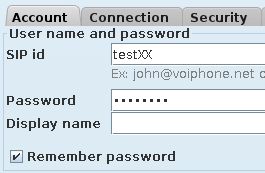
\includegraphics[scale=1]{img/sip_account.png}
  \caption{Základní informace o~účtu.}
  \label{fig:sip_account}
\end{figure}
\begin{figure}[H]
  \centering
  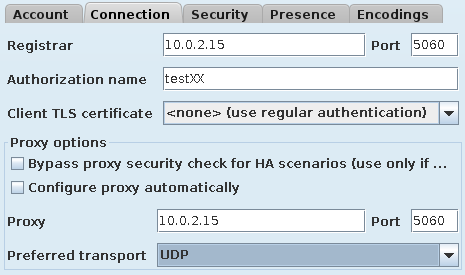
\includegraphics[scale=1]{img/sip_connection.png}
  \caption{Informace o~připojení, přihlašovací jméno k~ústředně a proxy.}
  \label{fig:sip_connection}
\end{figure}
\begin{figure}[H]
  \centering
  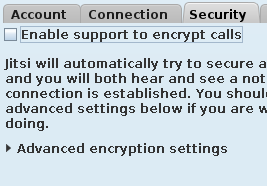
\includegraphics[scale=1]{img/sip_security.png}
  \caption{Deaktivace zabezpečení hovoru.}
  \label{fig:sip_security}
\end{figure}
    a potvrďte tlačítkama {\bf Next $\rightarrow$ Sign in}.
    \item Tímto jste provedli registraci k ústředně. Pokud jste vše nastavili správně, mělo by se v~pravém sloupci zobrazit \emph{SIP Online}.
    \item Zastavte zachytávání provozu v~programu Wireshark na obou počítačích a uložete zachycenou komunikaci do souborů \texttt{cv4-registerU-pcA.pcap} a \texttt{cv4-registerU-pcB.pcap}. Tyto soubory budete odevzdávat.
	\item Buď na PC-A nebo na PC-B vyfiltrujte SIP komunikaci ze zachyceného provozu, analyzujte registraci k ústředně a doplňte do protokolu požadované údaje z~paketu zaslaného ústředně (PC-U), který obsahuje žádost o~registraci klienta Jitsi nainstalovaného na PC-A nebo PC-B.
\end{enumerate}


\subsection{Analýza hovoru přes ústřednu}
\begin{enumerate}
    \item Na PC-A i na PC-B znovu spusťte zachytávání paketů v aplikaci Wireshark tlačítkem 
\includegraphics[width=3mm]{img/ws_start.png}.
    \item Na PC-A (jako uživatel test01) zadejte v~aplikaci Jitsi do pole pro telefonní číslo SIP adresu uživatele test02: {\tt 1002@10.0.2.15}, kde místo {\tt 10.0.2.15} napište IP adresu počítače PC-U (ústředny). {\tt 1002} je telefonní klapka uživatele test02.
    \item Zahajte hovor z~PC-A na PC-B stisknutím tlačítka zeleného sluchátka. Po chvíli hovor ukončete.
	\item Zastavte zachytávání provozu v~programu Wireshark na obou počítačích a uložete zachycenou komunikaci do souborů \texttt{cv4-calloverU-pcA.pcap} a \texttt{cv4-calloverU-pcB.pcap}. Tyto soubory budete odevzdávat.
	\item Proveďte v~aplikaci Wireshark analýzu hovoru podobně jako u~peer-to-peer hovoru ({\bf Telephony $\rightarrow$ VoIP Calls $\rightarrow$ \bf Flow Sequence}).
    \item Zakreslete průběh spojení do grafu v~protokolu. Zkombinujte informace z~obou virtuálních počítačů (PC-A i PC-B) a do protokolu zaneste úplnou komunikaci všech
      tří stanic (PC-A, PC-B a PC-U). Uveďte, mezi kterými IP adresami a porty probíhá signalizace a mezi kterými přenos dat. Vyplňte, které protokoly se používají pro signalizaci a které pro přenos. Dále zjistěte, jaký kodek pro přenos hlasu byl použit.
\end{enumerate}


\section*{Odevzdávané soubory}
Zkontrolujte, zda máte všechny soubory které se budou odevzdávat:
\begin{itemize}
  \item \texttt{protokol4.pdf}
  \item \texttt{cv4-p2p-pcA.pcap}
  \item \texttt{cv4-p2p-pcB.pcap}
  \item \texttt{cv4-registerU-pcA.pcap}
  \item \texttt{cv4-registerU-pcB.pcap}
  \item \texttt{cv4-calloverU-pcA.pcap}
  \item \texttt{cv4-calloverU-pcB.pcap}
\end{itemize}

\section*{Ukončení práce v~laboratoři}
\begin{itemize}
	\item Do WIS-u odevzdejte vyplněný \texttt{protokol4.pdf} a všechny zachycené \texttt{pcap} soubory.
	\item Vypňete virtuální stroje a obnovte jejich snapshot vytvořený na začátku této laboratoře.
\end{itemize}
